\clearpage
\section{Problembeskrivelse}
\label{problemBeskrivelse}


%Her kan du skrive om din problembeskrivelse

I dette designprosjektet så skal det designes et Anti-Aliasing filter med en prunktprøvings frevkvens på $f_s = 3400$Hz. Et Anti aliasing filteer skal ha knekkfrekvens $f_c = 75\%$ av båndbreddegrensen $f_B$, dvs at $f_c \geq 0.75 \frac{f_s}{2}$. I tillegg så skal filteret ha en dempning på minst $10$dB ved $f_B = \frac{f_s}{2}$. Som et siste krav skal filteret påvirke signalet så lite som mulig i frekvensområdet $0 \leq f \leq 0.75 \frac{f_s}{2}$, dvs at filteret skal ha en maksimal dempning på $1$dB i dette området. En visualsering av kravene til filteret er vist i figur \ref{fig:krav}.

\begin{figure} [!h]
\centering
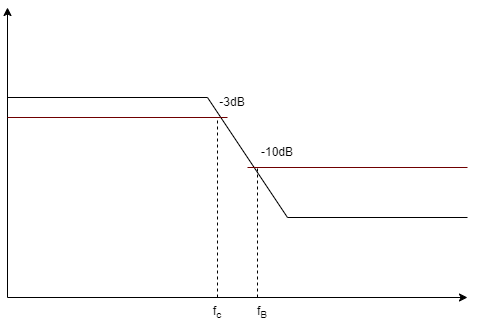
\includegraphics[width=0.7\linewidth]{Bilder/Anti_Aliasing_krav.drawio.png}
\caption{Et ideelt filter som tilfredstiller kravene til et Anti-Aliasing filter}
\label{fig:krav}
\end{figure}